\documentclass[a4paper]{article}

\usepackage[english]{babel}
\usepackage[utf8]{inputenc}
\usepackage{amsmath}
\usepackage{graphicx}
%\usepackage[colorinlistoftodos]{todonotes}
\usepackage[parfill]{parskip}
\usepackage{multirow}

\usepackage{hyperref}

%\usepackage{geometry} % to change the page dimensions
%\geometry{a4paper} % or letterpaper (US) or a5paper or....
\usepackage{booktabs} % for much better looking tables
\usepackage{paralist} % very flexible & customisable lists (eg. enumerate/itemize, etc.)
\usepackage{verbatim} % adds environment for commenting out blocks of text & for better verbatim
\usepackage{subfig} % make it possible to include more than one captioned figure/table in a single float

%%% HEADERS & FOOTERS
\usepackage{fancyhdr} % This should be set AFTER setting up the page geometry
\pagestyle{fancy} % options: empty , plain , fancy
\renewcommand{\headrulewidth}{0pt} % customise the layout...
\lhead{}\chead{}\rhead{}
\lfoot{}\cfoot{\thepage}\rfoot{}

%%% SECTION TITLE APPEARANCE
\usepackage{sectsty}
\allsectionsfont{\sffamily\mdseries\upshape} % (See the fntguide.pdf for font help)
% (This matches ConTeXt defaults)

\usepackage{listings}
\usepackage{color}

\definecolor{mygreen}{rgb}{0,0.6,0}
\definecolor{mygray}{rgb}{0.5,0.5,0.5}
\definecolor{mymauve}{rgb}{0.58,0,0.82}

\lstset{ %
  backgroundcolor=\color{white},   % choose the background color; you must add \usepackage{color} or \usepackage{xcolor}
  basicstyle=\footnotesize\ttfamily,        % the size of the fonts that are used for the code
  breakatwhitespace=false,         % sets if automatic breaks should only happen at whitespace
  breaklines=true,                 % sets automatic line breaking
  captionpos=b,                    % sets the caption-position to bottom
  commentstyle=\color{mygreen},    % comment style
  deletekeywords={...},            % if you want to delete keywords from the given language
  escapeinside={\%*}{*)},          % if you want to add LaTeX within your code
  extendedchars=true,              % lets you use non-ASCII characters; for 8-bits encodings only, does not work with UTF-8
  frame=single,                    % adds a frame around the code
  keepspaces=true,                 % keeps spaces in text, useful for keeping indentation of code (possibly needs columns=flexible)
  keywordstyle=\color{blue},       % keyword style
  language=Java,                 % the language of the code
  morekeywords={*,...},            % if you want to add more keywords to the set
  numbers=left,                    % where to put the line-numbers; possible values are (none, left, right)
  numbersep=5pt,                   % how far the line-numbers are from the code
  numberstyle=\tiny\color{mygray}, % the style that is used for the line-numbers
  rulecolor=\color{black},         % if not set, the frame-color may be changed on line-breaks within not-black text (e.g. comments (green here))
  showspaces=false,                % show spaces everywhere adding particular underscores; it overrides 'showstringspaces'
  showstringspaces=false,          % underline spaces within strings only
  showtabs=false,                  % show tabs within strings adding particular underscores
  stepnumber=2,                    % the step between two line-numbers. If it's 1, each line will be numbered
  stringstyle=\color{mymauve},     % string literal style
  tabsize=2,                       % sets default tabsize to 2 spaces
  title=\lstname                   % show the filename of files included with \lstinputlisting; also try caption instead of title
}


\usepackage[nottoc,notlof,notlot]{tocbibind} % Put the bibliography in the ToC
\usepackage[titles,subfigure]{tocloft} % Alter the style of the Table of Contents
\renewcommand{\cftsecfont}{\rmfamily\mdseries\upshape}
\renewcommand{\cftsecpagefont}{\rmfamily\mdseries\upshape} % No bold!


\title{SSAS-E2013}
\author{Team 6:\\Christian Lyngbye clyn@itu.dk\\Jacob Fischer jaco@itu.dk\\Rasmus Greve, Ivaylo Sharkov}

\begin{document}
\maketitle

\newpage
\tableofcontents

\newpage
\section{Introduction}
This report documents the project we completed where the objective was implementing a secure system based on a hypothetical customer's requests.

Rather than focus on the common documentation of software systems where the methods of development are described including the analysis and design of the system, the report is focused on risks, threats and vulnerabilities in the system we developed and the countermeasures we found to mitigate the risks.

The report is structured according to the 3 pillars of Software Security\cite{McGraw2006}. 
The first pillar Risk Management is addressed in the Strategy section \ref{sec:strategy}.

For the second pillar touchpoints, we have written several sections.

The specification of the system is described in section \ref{sec:specification} where we address the touchpoints of abuse cases and security requirements.

Next is the architecture in section \ref{sec:architecture} where we describe the technologies we have used and address the touchpoints: security operations, risk analysis and code review.

In section \ref{sec:testing} we describe the test plan that we created and how we address the risk-based security tests touchpoint. We also try to prove that we have implemented the specification.

The final touchpoint penetration testing is addressed in section \ref{sec:hacking} where we tried attacking the systems of the other teams. 

The third and final pillar Knowledge is discussed in section \ref{sec:discussion}.



%We start by describing our strategy for the architecture. We try to cover the 7 touchpoints except the code review.
%because we had trouble finding tools to do this. 

\section{Strategy}\label{sec:strategy}
By defining our strategy clearly and sharing it with our users, we hope to align our strategy with our business and technology.

We start by listing our goals and afterwards we will define how and why we expect to reach them.

\begin{itemize}
\item
We hope to engage our users in a new social platform based on their interests.
\item
The brand should build trust with the users over the long term so they keep coming back.
\end{itemize}

% how
We wish to achieve our goals by providing the following features to our users:
\begin{itemize}
\item Easy signup with design that provides high quality features with as few clicks as possible.
\item Adding and removing of friends and romances using an intuitive user interface
\item An easy way of adding and removing hobbies from your profile
\item Users can choose from a long list of social hobbies and find others with the same interests.
%\item Full data ownership: All data is owned by the users and should be easy to export and reuse.
\end{itemize}

\subsection{Risk Analysis and Management}
The business context is an application developed by a small enterprise with public customers with no contract of any sort. We provide a rudimentary service level agreement though there is no consequences if it is compromised. Most of the analysis is based on experience from using similar applications or our projections of how prospective interviewees would answer our questions.
\subsubsection{Business Goals}
We have decided on the following goals as paramount to our business operation with the web application. If any of these are not met, we consider it a severe threat to the integrity of our business.

\begin{table}[h!]
	\begin{tabular}{|p{10cm}|l|}
		\hline
		\textbf{Business Goal} & \textbf{Rank} \\ \hline
		The server must provide 99.5\% uptime   & \textbf{M} \\ \hline
		Sensitive user data is never compromised & \textbf{H} \\ \hline
		The application should be improved gradually by releasing new versions often & \textbf{L} \\ \hline
		Application must be live by October 4th 2013 &	\textbf{H}\\ \hline
		The application should be usable by a novice computer user on small screens (smartphones) as well as desktops & \textbf{M}\\ \hline
	\end{tabular}
	\caption{Business goals for our project. The goals are ranked with letters where L: low, M: medium and H: high}
	\label{tab:business_goals}
\end{table}

\subsubsection{Business Risks}
We have analyzed the business risks of the project and determined their impact which we have imagined as they would be for a small size enterprise.
\begin{table}[h!]
\begin{tabular}{| p{4cm} | p{3cm} | l | p{3cm} |}
\hline
\textbf{Business Risk} & \textbf{Indicators} & \textbf{Likelihood} & \textbf{Impact} \\ \hline
Data loss & Reports of service outage & L & Loss of potential users\\\hline
A user is subject to social engineering & Reports of peculiar activity & H & Damage to brand \\\hline
Vulnerabilities in the system & High amount of breaches & H & Unintended downtime and higher development costs \\\hline
Application delayed & System features are implemented late & M & Late return on investment \\\hline
\end{tabular}
	\caption{Business risk analysis for the social network system with impacts.}
		\label{tab:business_risk_analysis}
\end{table}

\subsubsection{Technical Risks}
The technical risks are characterized by their probability and effect on the system in table \ref{tab:risk_analysis}. We have also identified risks in making the system too secure.

\begin{table}[h!]
	\begin{tabular}{| p{5cm} | p{5cm} | l | l |}
		\hline
		\textbf{Risk} & \textbf{Indicator} & \textbf{L} & \textbf{C}  \\ \hline
        %User login bruteforcing & Repeated login attempts in logs & M & 6 \\ \hline
        %TR5 & SQL injections & 80\% & 9 & Prepared statements and input sanitization \\ \hline
        %User session hijacking & Reports from users of peculiar behavior & M & 4 \\ \hline
        Old libraries and platforms provide an easy target & Unauthorized access and several published vulnerabilities & H & 9 \\\hline
        Hardware failure & Reports of downtime & L & 5 \\ \hline
        Security is not part of system architecture design & Unauthorized access & M & 7 \\ \hline
		Security safeguards slows down user experience & Too many interactions & L & 3
		\\ \hline
		Non human users spam the system with irrelevant data & Garbled input with common words and quick repetitions of requests & H & 5
				\\ \hline
	\end{tabular}
	\caption{Risk analysis for the social network system with mitigation strategies. L: Likelihood that it will occur. C: Consequences on a scale from 1 to 10}
	\label{tab:risk_analysis}
	

\end{table}



In table \ref{tab:goal_to_risk_relationship} the business and technical risks are synthesized. The technical risks are from table \ref{tab:risk_analysis}.
\sffamily
\begin{table}[h!]
	\begin{tabular}{| p{4cm} | p{4cm}| p{4cm} |}
    \hline
   	\textbf{Business goals} & \textbf{Business Risk} & \textbf{Technical risk} \\ \hline
	Sensitive user data is never compromised & Vulnerability in the system & Old libraries and platforms provide an easy target \\ \hline
    The server must provide 99.5\% uptime & Data loss &  Hardware failure \\ \hline
    %\multirow{4}{4cm}{The web server is breached at most twice throughout the project period} & \multirow{4}{4cm}{Vulnerabilities in the system} & TR5 & SQL injection \\ & & TR8 & Replay attack \\ & & TR9 & Cross-site request forgery \\ & & TR12 & Cross-site scripting (XSS) \\ \hline    
    Application must be live by October 4th 2013 & Application delayed &  Security is not part of system architecture design \\ \hline
    The application should be usable by a novice computer user on small screens (smartphones) as well as desktops & A user is subject to social engineering & Security safeguards slows down user experience. Non human users spam the system with irrelevant data \\ \hline
    \end{tabular}
    \caption{Goal-to-risk relationship table.}
	\label{tab:goal_to_risk_relationship}
\end{table}

\rmfamily

\subsubsection{Mitigations}
We have ranked the risks and provide our proposals for mitigation.
\begin{description}
\item[Vulnerability in the system]
Use supported third party libraries and continuously check and update the technologies used in order to keep all parts of the software secure.
% to avoid the compromise of sensitive user data by Securing the Weakest Link.


%By assigning clients user credentials we can identify them and separate them into different roles that we might need and do \textbf{Separation of Privilege}.

\item[Data loss]
We can do backups of the database and encrypt it.

\item[Application delayed]
If we make a plan with milestones including scopes that gives an idea of what we hope to accomplish we can use this as an indicator of our progress.
Then we can decrease the scope or increase the work effort to compensate.

\item[A user is subject to social engineering]
The system can provide warnings to users if they are leaving the site by clicking a link that has been written by users.

\end{description}

% why
%\begin{itemize}
%\item Reluctance to Trust
%\item Securing the Weakest Link
%\item Failing Securely
%\item Least Privilege
%\item Separation of Privilege
%By assigning clients user credentials we can identify them and separate them into different roles that we might need.
%\item Promoting Privacy
%\end{itemize}
%Confidentiality, Integrity, Availability

\section{System Specification}\label{sec:specification}
In accordance with the project description, we have defined our system as a web application where students can form friendly or romantic relationships with other students. The application should furthermore support administrative users, who are able to modify certain aspects of the system from a client's perspective. These requirements derive from the user stories presented in the project description. Throughout the project period, there has been three such sets of requests from the "customer".

We have considered each of these user stories and made corresponding use cases for the system, leading to functional requirements. Some of the user stories have related instead to non-functional requirements, and some again to security requirements.

In addition, we have specified a number of abuse cases, constituting a security-related counterpart to the use cases. Based on these, we have derived additional functional, non-functional and security requirements. Not all abuse cases have had equal impact on the final specification, as we have had to keep in mind the strategic prioritizations outlined in the Risk Management section.

\subsection{Use cases}
\begin{enumerate}
\item A user signs up as a student
\item A student views/edits his own information
\item A student requests a friendship with another student
\item A student approves a friendship request with another student
\item A student upgrades a friendship to a romance
\item A student views a student’s information when they are in a relationship
\item A student sends a "hug" to a student that they are in a relationship with
\item An administrator deletes an existing user
\item An administrator views the information of a user
\item A competing service imports public data from our application
\item Our application imports public data from a competing service
\end{enumerate}

\subsection{Abuse cases}
\begin{enumerate}
\item A malicious user runs arbitrary queries on the database by submitting SQL code through an input field
\item A malicious user injects a script into HTML content that is presented to other users
\item A malicious user fills the system with irrelevant data by automatically creating multiple user profiles with a self-repeating script
\item A malicious user with two profiles logs into two different sessions and attempts to induce a race condition in the system by having both profiles befriend each other simultaneously
\item An unauthorized third party is picking up a user's traffic by listening on the same network the user is connected from
	\begin{enumerate}
		\item The third party gains access to sensitive user data against the regulations of the privacy policy
		\item The third party gains access to the user's session ID, allowing the intruder to impersonate the user when communicating with the application
	\end{enumerate}
\item A person with access to an administrator's credentials wrecks havoc on the system by deleting multiple user profiles
\item A competing web service exposes malicious data, such as client-side executable code, when exporting to our application
\end{enumerate}

\subsection{Functional Requirements}
Most of the following functional requirements are derived from the use cases, to support the functionality that the customer has requested in the project description. 


\begin{enumerate}
\item A database model supporting users with the following data represented:
  \begin{enumerate}
  \item User
      \begin{enumerate}
      \item Username (this is necessary as the customer wants both proper name and email to be private information)
      \item Password
      \item Email
      \item First name
      \item Last name
      \end{enumerate}
  \item Hobbies
  \item Friends/romances
  \end{enumerate}
\item CRUD for users
	\begin{enumerate}
    \item Users should be able to view their own data
    \item Users should be able to view other users' data, filtered depending on their relationship with the given user
    \item Users should be able to edit their own data upon re-entry of their password (see security requirement 1)
    \item Admins should be able to suspend and restore user profiles (see security requirement 2)
    \end{enumerate}
\item User authentication
	\begin{enumerate}
	\item Captcha authentication on the user creation form
	\end{enumerate}
\item Admin authorization
\item Browse functionality for finding other users
\item Exposition of public data through a REST API
\item Support for importing public data from an external REST service into our own application
\end{enumerate}

\subsection{Non-functional requirements}
The following is our non-functional requirements to the system. These are derived from our business goals, one of which relates to uptime. Another of our business goals is to employ immediate mitigation against any attack we might be subject to throughout the project period.
\begin{enumerate}
\item The application is available through an HTTP connection 99.5\% of the time
\item A logging framework is enabled that allows the team to identify the underlying causes of any breaches that may occur
\end{enumerate}

\subsection{Security Requirements}
\begin{enumerate}
\item In order to prevent an intruder who has hijacked a user's session ID from tampering with the user profile itself, we require users to re-enter their password whenever they submit changes to their profile data.
\item In order to prevent people with access to an administrator's credentials from destroying user data in the system, an administrator is only able to suspend (and not delete, as per the use case) user profiles. Other administrators will then be able to restore the profile, in the case of a mistake. We feel that this is a good compromise, which does not stray too far from the original use case.
\end{enumerate}

\section{Architecture}\label{sec:architecture}


\subsection{Operations}
Our production server runs a Ubuntu distribution of Linux.
% and provides the access control for users' access to the file system.

There are assets that should be protected because we want to promote privacy:
\begin{itemize}
\item Database for the application
\item Log files for the application
\end{itemize}

\subsubsection{Frameworks and Technologies}
The following is a list of all the frameworks and technologies we have decided to use, with a short justification for each. In general we use open source technologies that promote awareness about security issues.

Frameworks:
\begin{description}
\item[JSF2] This is the recommended dynamic web page technology for this course, which makes help more readily available. In addition, we are all fairly experienced with Java, and one person on the team has prior experience with JSF. It provides protection against XSS and CSRF. 
\item[Hibernate 3] is a library that provides ORM and can encapsulate database access in transactions and maps objects to relations.
\item[JUnit and Selenium with Selenide] for testing our application. JUnit provides a unit-testing framework for Java, which Selenium integrates with. Selenide is a framework for running tests for a web application through the browser.
\item[Commons Logging]
Tomcat supports commons logging and we use this to track user activity in an audit log.
\end{description}
Technologies:
\begin{description}
\item[Apache Tomcat 7.0.26] This is a lightweight application server for Java web applications that supports Servlet 3.0 and HTTP 1.1. It is the recommended server technology. 
\item[PostgreSQL 9.1.9] is a RDBMS that provides extensive functionality like auto generated id sequences and fine-grained access control of database operations for users. The developers provide a list of security issues \footnote{\href{http://www.postgresql.org/support/security/}{http://www.postgresql.org/support/security/}} and we have considered that the version we chose is safe.
\item[UFW] The Uncomplicated Firewall, is a straightforward firewall implementation for Linux that provides easy configuration of port filtering/blocking etc.
\item[Uptime Robot] This is a uncomplicated and free SaaS that monitors websites for downtime and sends email if they are unresponsive.
\item[Snort] Snort is an Intrusion Detection System that logs intrusions using tcpdump.
\end{description}

\subsection{Architecture Risk Analysis}


\subsubsection{Attack Resistance Analysis}
We found the following historic attacks on applications.

\begin{table}[h!]
	\begin{tabular}{| l | p{4cm} | l | l | p{5cm} |}
		\hline
		\textbf{ID} & \textbf{Threat} & \textbf{P} & \textbf{C} & \textbf{Possible mitigation} \\ \hline
		TR1 & User gives away password & 2\% & 6 & Educate users. Restrict user privileges. \\ \hline
        TR2 & Admin gives away password & 0.1\%  & 10 & High requirements for admin hiring \\ \hline
        TR3 & Admin login bruteforcing & 50\% & 10 & Password requirements and login throttling \\ \hline
        TR4 & User login bruteforcing & 30\% & 6 & Password requirements and login throttling \\ \hline
        TR5 & SQL injections & 80\% & 9 & Prepared statements and input sanitization \\ \hline
        TR6 & Admin session hijacking & 10\% & 8 & Encrypted connections \\ \hline
        TR7 & User session hijacking & 1\% & 4 & Encrypted connections \\ \hline
        TR8 & Replay attacks & 1\% & 3 & Use nonces \\ \hline
       	TR9 & Cross-site request forgery & 1\% & 8 & Use nonces \\ \hline
        TR10 & Hardware failure & 5\% & 8 & Multiple servers and data backups \\ \hline
        TR11 & Server loses internet connection & 0.1\% & 5 & Multiple servers and/or connections \\ \hline
        TR12 & Cross site scripting (XSS) & 5\% & 8 & Input sanitazion and validation \\ \hline
	\end{tabular}
	\caption{Threat analysis for the social network system with mitigation strategies. P: Probability in percent. C: Consequences on a scale from 1 to 10}
		\label{tab:threats}
\end{table}



We have chosen this prioritization of threats by looking at the probability and consequenses of each of them as well as estimating how complicated it is to implement the mitigation strategy.



\subsubsection{Ambiguity Analysis}

We didn't validate user input so all the sanitized text was saved to the database text fields. 

We experienced some issues dropping our database which we guessed was because the special characters in the text fields blocked the command from execution.

Here are some examples of malicious user input:
\begin{verbatim}
\\etc/passwd
any\r\nSet-cookie: Tamper=2918187384565502119
"><script>alert(1);</script>
\end{verbatim}

Furthermore we didn't have any password rules.

\subsubsection{Weakness Analysis}
We ran the vulnerability scanner called w3af against our own application in order to find weaknesses.

w3af is in the words of the creators a "Web Application Attack and Audit Framework". It is open source and developed in python. It is built as a plugin framework where each known vulnerability to test, is contained as a plugin. This makes it easy to change what is tested and carefully conduct a specialized attack against a web application where you know which tools and frameworks run underneath.

We setup the tool to check with the OWASP Top 10 profile with the following plugins that check for vulnerabilities.

\begin{verbatim}
xsrf, htaccessMethods, sqli, sslCertificate, fileUpload, mxInjection, 
generic, localFileInclude, unSSL, xpath, osCommanding, remoteFileInclude, 
dav, ssi, eval, buffOverflow, xss, xst, blindSqli, formatString, 
preg_replace, globalRedirect, LDAPi, phishingVector, frontpage, 
responseSplitting
\end{verbatim}
     
We found vulnerabilities in the public web pages:
\begin{verbatim}
 The following scripts are vulnerable to a trivial form of XSRF:
 - http://team6.bollgreve.dk/ssase13/f/profile.xhtml
 The following scripts allow an attacker to send POST data as query 
 string data (this makes XSRF easier to exploit):
 - The URL: http://team6.bollgreve.dk/ssase13/f/signup.xhtml is 
vulnerable to cross-site request forgery. It allows the attacker to 
exchange the method from POST to GET when sendin data to the server.
\end{verbatim}
This is due to the JSF libraries that only partially protect against Cross(X) Site Request Forgery. This is a weakness in the platform we have chosen.
\begin{verbatim}
 The URL: http://team6.bollgreve.dk/ssase13/f/profile.xhtml is 
vulnerable to cross-site request forgery.
 An unidentified vulnerability was found at: 
 "http://team6.bollgreve.dk/ssase13/f/profile.xhtml", 
 using HTTP method GET.  The sent data was:
 "id=d%27kc%22z%27gj%27%22%2A%2A5%2A%28%28%28%3B-%2A%60%29". 
 This vulnerability was found in the requests with 
 ids 1016 to 1017 and 1019.
\end{verbatim}

We are not sure what the unidentified vulnerability mentioned is but this is one of the requests:
\begin{verbatim}
========================================
Request 1017 - Sat 14 Dec 2013 01:09:11 AM CET
========================================
GET 
http://team6.bollgreve.dk/ssase13/f/profile.xhtml?id=27854292 
HTTP/1.1
Accept-Encoding: gzip
Accept: */*
User-Agent: w3af.sourceforge.net
Host: team6.bollgreve.dk
Cookie: JSESSIONID=CC4B00E98F4083C6CB66E1B5A4974676
Referer: http://team6.bollgreve.dk/
\end{verbatim}

If we look up the page manually we are shown an empty profile page so we cannot confirm that this is a vulnerability. However it proves that a vulnerability scanner is a powerful tool to extend abuse cases.  We are aware that the tool might only catch the most critical exceptions and a thorough penetration test would be better.

To help identify weaknesses we drew a Forest View diagram as seen in Figure \ref{fig:forest_view}.

\begin{figure}[h!]
\centering
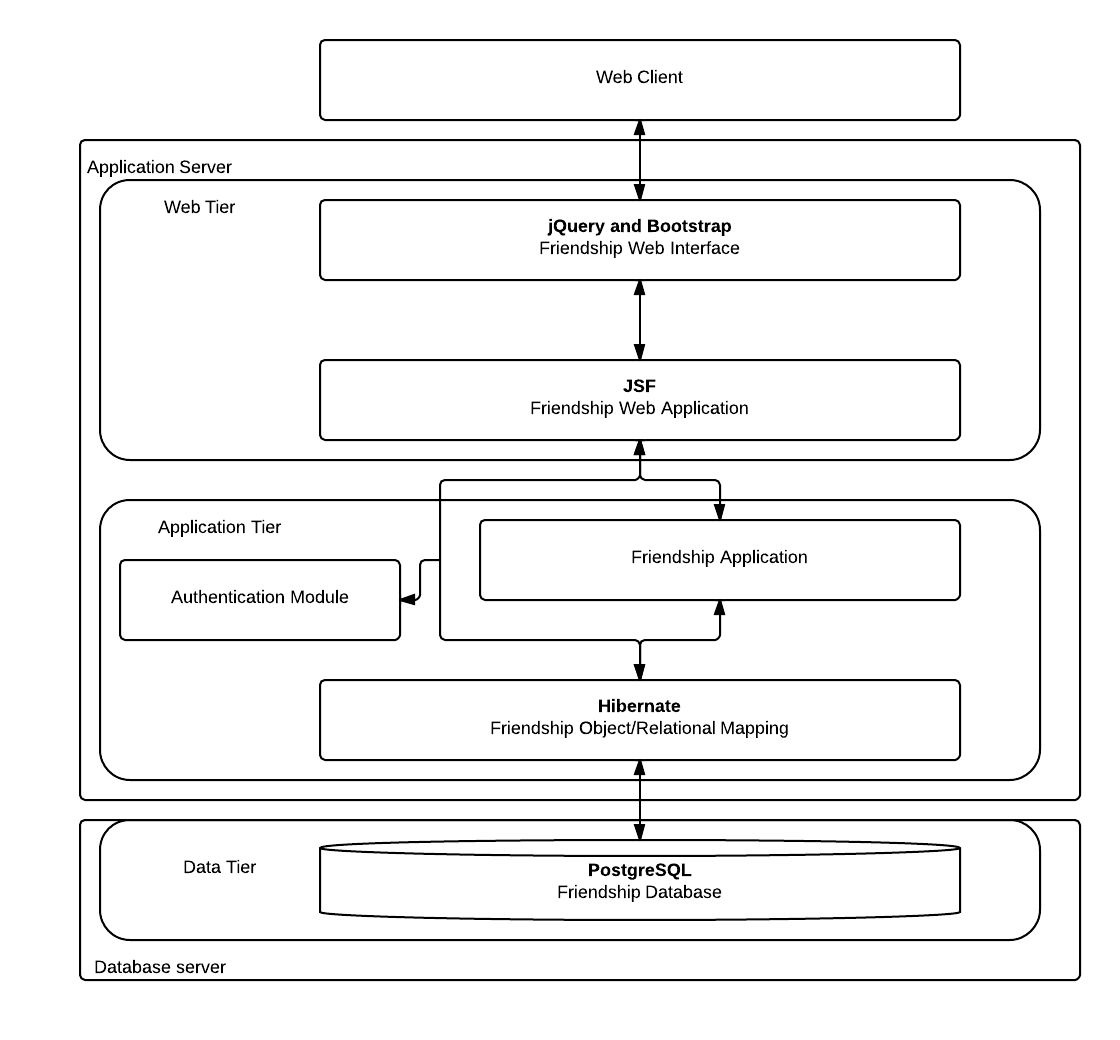
\includegraphics[scale=0.35]{ForestView}
\caption{Forest View diagram}
\label{fig:forest_view}
\end{figure}

The communication between the web client and the application server is not protected \cite{sins2009} because it is plain text http packets sent over the network. This weakness is usually exploited by a 'man-in-the-middle' who can follow an attack pattern that spoofs ARP packets in order to intercept the requests to the server and read usernames and passwords.

\subsubsection{Development Safeguards}
Based on the probability and consequence of the threats we have chosen to protect the implement safeguards against the following threats:
\begin{description}
\item[SQL injections] By encapsulating database queries in prepared statements. Hibernate, which we use for ORM, renders any SQL injection attempt useless by supporting prepared statements and parameterization.
\item[XSS attacks] JSF2 provides safeguards protecting against this.
\item[Race conditions] We can avoid deadlock by using transaction in Hibernate. 
We have also taken measures to protect against race conditions, one of the sins covered in \cite{sins2009}. This is for the most part a question of making sure to write re-entrant code in critical sections where race conditions could be a threat to the integrity of our data. It is also inherently supported at the database layer by transactions in Hibernate.
\item[Login bruteforcing] Password requirements should prevent the most common low security passwords. If the database is exposed all passwords are hashed using the
\textbf{SHA-256} algorithm with a randomly generated 4 character salt for every user.
%At this point in time it is regarded as a considerably secure hashing algorithm.
\item[Non human users spam the system with irrelevant data] Implementing captcha's prevents non humans from filling out forms.
%\item[Admin subject to social engineering]
\end{description}

%TODO: Does JSF protect against XSS attacks?

One of the functional requirements that was required was to protect address and real names. This required us to create a trust zone for the application that authenticates users based on their role (user/admin). 

We use session objects to control access to pages based on a black list of which pages are public. By designing it this way we always protect new pages so it is not necessary to register them in a white list. 

The following pages are unprotected:
\begin{description}
\item[login.xhtml] - default landing page
\item[signup.xhtml] - sign up page
\item[userList.xhtml] - list of all users
\item[profile.xhtml] - a users profile
\item[alienprofile.xhtml] - an externally imported profile
\end{description}

The authentication module in the forest view shown in figure \ref{fig:forest_view} is an extended JSF Phase listener that overrides the afterPhase method to check for login. Otherwise it redirects to the login page.
Furthermore there is a filter that protects against accessing the web pages outside the JSF servlet.  
  

Based on the priorities of the Risk Management section, as well as the previously listed abuse cases, we have derived the following security requirements to our application.



We have chosen not to safeguard the network traffic vulnerability by requiring the application to use SSL, because the probability of the attack is low. The impact of an attacker getting access a password is also low because the password cannot be changed. Furthermore we don't regard full names and addresses to have a critical impact if exposed.

% as although it would provide good protection against abusive users sniffing packages on an open network, we have decided not to pursue this for a variety of reasons. 

There are other circumstances regarding certificates. Our server doesn't have an assigned domain name which is required for getting a signed certificate. Furthermore most signed certificates cost money to request.
%It is also not a completely trivial task to set up a certificate, and it is further complicated by the absence of a domain name to register it with. 

An alternative is to create a self-signed certificate. It would cause a considerable reduction in usability, because most browsers warn users against entering sites with non-signed certificates. 

Instead of creating a self-signing a certificate we have modified our functional requirements to mitigate this particular abuse through alternative means.

We needed to integrate with another team bu they used a self signed certificate. This made it necessary to create our own SSLSocketFactory. By downloading the certificate and importing it into a keystore, see figure \ref{fig:ssl_keystore} we could deploy it inside our application. 
\begin{figure}[h!]
\caption{Custom SSL keystore}
\label{fig:ssl_keystore}   
\begin{lstlisting}
KeyStore keyStore = KeyStore.
  getInstance(KeyStore.getDefaultType());
keyStore.load(keyStoreInput, "team10".toCharArray());
TrustManagerFactory tmf = TrustManagerFactory.
  getInstance(TrustManagerFactory.getDefaultAlgorithm());
tmf.init(keyStore);
SSLContext ctx = SSLContext.getInstance("TLS");
ctx.init(null, tmf.getTrustManagers(), null);
return ctx.getSocketFactory();
\end{lstlisting}
\end{figure}
This way we could set it as a trusted certificate by hardcoding the hostname verifier to the IP we knew the team used, see figure \ref{fig:ssl_verifier}, because otherwise the HTTPS client would fail.

\begin{figure}[h!]
\caption{Imported SSL Verifier}
\label{fig:ssl_verifier}   
\begin{lstlisting}
urlcon.setHostnameVerifier(new HostnameVerifier()
{
  @Override
  public boolean verify(String hostname, SSLSession session)
  {
    if (hostname.equals("192.237.201.172"))
      return true;
    return false;
  }
});
\end{lstlisting}
\end{figure}


%Securing traffic with SSL also makes it harder for clients to communicate with our application through the REST API. 

%\begin{itemize}
%\item 
%\item Database access credentials are never stored in any source code repository
%\item The database is always accessed in a manner that protects against SQL injection
%\item The application guards against cross-site scripting
%\item Logfiles on the web server are only accessible with root permissions
%\item All input from users and other web services is validated and/or sanitized
%\end{itemize}


% \ref{sec:appendix:racecondition} This "test" is really bad...


We do not claim to protect against XSRF attacks so we did not have a safeguard.

We validate the text input with the following regular expressions. We use the first one for usernames and other inputs that are one word only, and the second one for input where multiple words are allowed. Finally our passwords require small and capital characters as well as numbers.
\begin{verbatim}
STRING_REGEX = "^\\w+$";
WORDS_REGEX = "^(\\w+\\s?)+$";
PASSWORD_REGEX = "^(?=.*[a-z])(?=.*[A-Z])(?=.*[0-9]).{6,}$";
\end{verbatim}

\subsubsection{Operational Safeguards}
Based on a common set of security design principles \cite{princ} that we have chosen from we have addressed threats in the operations.

\begin{description}
\item[Least Privilege] 

We have disabled remote login for the root user. Users are only given the necessary privileges to the file system so we protect log files from malicious users.
The application server and database runs each with their respective user that is only used for that process. However we needed to host the application on port 80 so we configured it using another tool called authbind.
% TODO find tool give root access to the application server because it needs to run on port 80.

The database user/role for the database creation is different from the user that is used by the application server. 
%By applying this practice we give the application the least possible privilege to the database to protect our database from being dropped.

We have created users for each member of the teamn in a group with superuser rights. Furthermore there are users created for the web application and database.
This ensures that we can withdraw rights if necessary without losing access to the system.
This way we have restricted access to the database by only allowing the database user itself to connect as a client without password.

\item[Reluctance to Trust]
We only store the unique password to the database for the application user on the server. We don't trust the confidentiality of our Version Control System.

\item[Promoting Privacy]
A firewall blocks requests on all ports except port 80 (HTTP) and port 6666 (SSH).

\item[Least Common Mechanism]
We configured the SSH daemon to listen on port 6666 instead of 22 because this might prevent attackers from bruteforcing login.

\item[Fail Securely]
There is no need to expose information about the software we use so we filter out 404/500 error codes in our application to show our custom error page.
\end{description}

\subsubsection{Project Tools}
We have chosen to use the following tools to assist us in our project process.
\begin{itemize}
\item \textbf{Git} is our chosen tool for source control, since it is easy to use and gets the job done, and Github is a decent platform for hosting source code on. We used the Github issue tracking system to keep track of new feature requests as well as bugs.
\item \textbf{Google Docs} is what we use for taking notes and making on-the-fly documents, spreadsheets or presentations that we might need throughout the project. It is very easy to share things here, but the text processing tool is not that powerful, so it is not where we write our report.
\end{itemize}
We did informal code review before each milestone by checking the issues that we had created in Github and the quality of the implementation as a group.

\section{Testing}\label{sec:testing}
In order to ensure that our service works as intended and do not have any immediate flaws we have conducted a series of automated and manual tests. 
The tests were developed in priority according to the risks and abuse cases that we have designed.

\subsection{Test plan}
Our strategy for testing was twofold: We would like to prove that the functionality of all components worked and we wished to test the overall quality of the system using system tests.

\subsubsection{Testing objectives}
We have had two objectives with our tests, both to confirm that the required features are correctly implemented and working (e.g. validation testing), but also that any error cases or abuse cases result in error messages or at least correct behavior (i.e. defect testing)

\subsubsection{Features to be tested}
We have aimed at testing as many features as possible, but core features haven been tested more thoroughly than peripheral secondary features due to the strict and early deadline. Drawing the line between core and peripheral features is tough and might seem a bit arbitrary, but we have aimed at prioritizing features related to our own service over the exposed REST API as well as the REST integration.

Our automated tests are aimed at the following components:
\begin{itemize}
\item Signup
\item Login
\item Friends relation features
\item Hobbies
\item Updating profile
\item Using the service w/o login
\end{itemize}
\subsubsection{Testing techniques}
We wanted to test as thoroughly as possible and ideally also include unit tests, but this was not possible due to the time constraints.
We have used the following testing techniques:
\begin{itemize}
\item Grey box testing
\item Manual system tests
\end{itemize}

%\subsubsection{Static Testing} Static testing is testing of a component or specifications without execution of that software.  This is usually done as soon as acceptance criteria or business requirements are ready for review before code implementation such as conflicting rules, invalid data types, redundant process just to name a few. 
%
%\subsubsection{Component Testing}
%Component level testing focuses on the functionality of each component being developed.  This is  crucial where different components are being developed before they are integrated together as one system.
%
%Entry Criteria
%
%Component Testing may commence when the following criteria has been satisfied:
%All code has been unit tested and passed.
%Test environment including software has been setup and configured correctly.
%Business requirements and test cases are up to date as per user story.
%
%Suspension Criteria
%
%Component testing will be suspended under the following condition:
%Critical error(s) found preventing test completion.
%Change of business requirements.
%Change of environment components or technology including different version.
%
%Resumption Criteria
%
%Component testing will resume when the following criteria are met:
%All issues in suspension criteria have been resolved or mitigated.
%New software build has been redeployed.
%
%Exit Criteria (Test Completeness)
%
%Component testing can be considered complete when the following conditions have been met:
%All requirements have been tested without Critical or Medium severity defects.
%\subsubsection{System Testing}
%The purpose of the system testing is to validate that the complete and integrated system complies with functional requirements and business requirements.
%
%Entry Criteria
%
%System testing may commence when the following criteria have been satisfied:
%Component Testing has been completed.
%No change to business requirements and test cases are up to date.
%Scenario based test cases have been reviewed.
%
%Suspension Criteria
%
%System Testing will be suspended under the following condition:
%Critical error(s) found affecting functionality of the whole system.
%Change of business requirements.
%
%Resumption Criteria
%
%System Testing will resume when the following criteria have been satisfied:
%All issues in suspension criteria have been resolved or mitigated
%
%Exit Criteria (Test Completeness)
%
%System Testing will be considered complete when the following conditions have been met:
%All High and Medium priority requirements have been tested without Critical or Medium severity defects.
%
%Business owner and/or business user have been notified with any remaining defects and understand the risks or limitations of current release.
%
%User Acceptance Testing 
%
%UAT is a formal testing with respect to user needs, business requirements and expectations.  The idea here is to gain confidence from business owner on the software being developed.  Although it is not mandatory business owner(s) and/or business user(s) are expected to produce his/her own test scenarios.
\subsection{Tools and Frameworks}
A testing tool we found fitting to use for system tests is Selenium\footnote{Selenium webpage: http://www.seleniumhq.org/} and Selenide\footnote{Selenide github page: https://github.com/codeborne/selenide} with JUnit. Selenium allows us to script test cases which input data and submit forms on the webservice using the test structure from JUnit.
When the tests are running, Selenium starts firefox and executes all the commands entered by looking through the DOM for elements to enter data, click buttons or verify the values.

Creating an automated test suite makes development and especially refactoring a breeze since whenever something is changed it is easy to verify that everything that worked beforehand, still works. It should be noted that we of course don't assume that our test cases cover everything, but they still give a good indication of whether or not a change has broken functionality.

\subsection{System Test Cases (Grey-box Test)}
We use grey box testing to do system testing, meaning that we mainly do white box testing to test use cases, but use our knowledge of the implementation to write the abuse cases so that they would fail if they could.

\subsubsection{Signup}
The signup form must be visible and usable when you are not signed in, otherwise it wouldn't be of much use. There is a requirement that user handles be unique, and that passwords must be at least 6 characters long and contain lowercase and uppercase letters as well as numbers.

The signup form also has a CAPTCHA\footnote{CAPTCHA: Completely Automated Public Turing test to tell Computers and Humans Apart} test which by the intention of the CAPTCHA we won't be able to automatically enter correctly.

The only tests we have been able to automate regarding signup is illegal password and wrong CAPTCHA. In the code the handle is tested for uniqueness after the CAPTCHA has been validated, so this feature has been tested manually.

\subsubsection{Login}
The login form has been tested by inputting valid and invalid login information and testing that we are and aren't logged in respectively. We have also implemented an automatic SQL injection test to ensure that it is not possible to execute SQL statements by putting them into the form fields.

\subsubsection{User relations}
Our user relations test is a validation test to ensure that all the required features are implemented and working. The following features are tested:
\begin{itemize}
\item View list of friends
\item Request friendship
\item Accept friendship
\item Remove friendship
\item Start romance
\item End romance
\end{itemize}

\subsubsection{My profile}
It has been tested that you can enter and edit information about your own name, surname and address. All features have also had abuse cases tested where XSS attempts and SQL injection attempts has been tested and proven to not work.

\subsubsection{When not logged in}
It is possible to use our webservice without logging in. This has required us to test and ensure that only the publicly available information is available to users that are not logged in.
We test that anonymous users cannot request friendships or delete users, but that they can see a list of users and view their profile.
On the profile page we test that only the handle and hobbies are visible and name, address and recent activities are hidden.

\subsubsection{Manual tests}
The previously mentioned test cases have been automated using our testing framework Selenium, since Selenium is designed for HTML DOM testing. This made it less useful for testing our REST API, which instead has been tested manually and of course implicitly by the team consuming our API (team 10).

\section{Hacking}\label{sec:hacking}
Penetration testing is the process of conducting a test of a system that is partially or fully implemented and running preferably in the production environment, in order to get as realistic a test setting as possible.

The goal of the test is to uncover security problems in the application by actually trying to attack the running application using any number of techniques. This exercise is commonly executed by security experts that have experience in discovering vulnerabilites that they can exploit.
% about the general concepts of hacking and attacking, and who understand the proper way to exploit weaknesses. 
One big step to hack an application is to establish a bridgehead on the server. 

Any vulnerability on the server can work as a bridgehead and the application can only be as secure as its weakest link.

One part of finding vulnerabilities to exploit is to discover which technologies and frameworks that are run on the server an application uses. Over time software tends to degrade in security and one particularly valuable piece of information is the particular version a technology has. 
Using this information it is possible to look in bug databases\cite{CVEdb} to search for vulnerabilites that might be possible to exploit.

\textbf{Automated testing}
Tools have been created to aide the security expert in her analysis or to help novice security testers. Basically two kinds of tools exist; static analysis tools and dynamic testing tools.
The static tools work by inspecting either the source code of the application if this is available, or binaries/decompiled binaries, trying to find common implementation errors in the application that can be exploited by malicious users or simply triggered by unknowing normal users.
The dynamic tools work by inputting lots of different data in all data-entry points in the application. Usually edge-case data is used such as 0, 1 and 2,147,483,647 for numbers and empty or very long strings maybe containing special characters or for string inputs.

\subsection{Discovery with NMap scan}
We ran NMap scans on the servers of the teams. The interesting points follow
\begin{itemize}
\item MySQL 5.5 is available running on port 3306 for team 5, 7 and 10
\item SvnServe is available on port 3690 for team 7
\end{itemize}


\subsection{Social engineering attack}
A social engineering attack requires some knowledge and analysis of the setting, system and people you want to attack.

The setting at hand is that we are among a set of teams all implementing and trying to secure a webservice which must be "handed in" and shown off to a teacher and possibly the TA. This implies that the people in the teams all trust both the teacher and the TA. We have observed that most of us do not remember the name of the TA off the top of our heads and need to look it up on the course blog.
We can use this knowledge to make a broad social engineering attack on all other groups attempting to obtain confidential information such as usernames and passwords for admin accounts.

The idea is to send an email to the entire class that looks and sounds official and says that it is from ``The TA of System Architecture and Security F2013". We assume that the students are not aware of the name of our TA and that they will trust that if we claim to be him in the email, they will believe us. The email will contain a request for login information to their webservice for an admin account that we need in order to evaluate the teams' progress.

We thought of performing this attack multiple times, but never found a good time to do it. With these kinds of attacks timing is key, and every time we thought about sending the mail we felt like the timing wasn't right and that it would definitely be identified as phishing by the other teams.


%\subsection{Penetration test of team 11}
%As part of the project we have conducted a penetration test on another groups web service.

%Our attempt at a penetration test consist of us using a dynamic pen-test tool called w3af on the application of team 11.
%We cannot use a static analysis tool since we do not have access to neither source code nor binary code as everything is well hidden on the webserver. To perform the best possible penetration test we have attempted to get the source code from their server, but they seem to have configures their firewall well and closed any holes that we have been able to think of. Given other circumstances a dictionary password breaking attack could have been performed in order to try to take over the server, but in this case all forms of DoS attacks are disallowed.


%\textbf{Attacking team 11}
%The webapplication that team 11 has made, "Raptor dating", seems to be

%About team 11
%w3af on team 11

\subsection{XSS attack on team 10}
\subsubsection{Description}
As part of the requirement to expose the publicly available data in our system to one or more of our competitors through a REST API, we saw a natural opportunity to try and inject malicious data into \textbf{their} systems. The basic idea was to have a piece of code in our REST service class replace the string exposed by the service when requesting a particular hobby with a different, pre-defined string, containing malicious data. This data would just be a text string, containing the HTML tag for JavaScript, executing an alert in the client's browser. This is just to demonstrate the vulnerability, as the ability to execute JavaScript originating from us on the clients of our competitor could lead to many kinds of attacks, particularly XSS.

Doing a bit of research, we found out that team 10 in particular might be vulnerable to this kind of attack. During conversations with them about how best to exchange data through a REST API, we learned that they stored the interests (hobbies) of their users in comma-separated text strings. At this point we also applied a dose of social engineering by explaining to them in detail how they might consume our web service from their application, in an attempt to get them to implement their client as naively as possible.


\subsubsection{Results}
See figure \ref{fig:xss_screencap} under chapter 9.4 in the appendix for graphical illustration of the results of this attack. As denoted in the figure, the Fishing hobby was the one we configured to result in malicious code rather than its innocent name in a string, whenever requested by a web server located on team 10's IP address. As can be seen, the user with the hobby correctly imports to team 10's "Friendship Portal", but the malicious string produced by the Fishing hobby is not displayed, and is not even present in the document's source. This indicates that team 10 did anticipate this kind of attack, and took the appropriate security measures by validating the data imported from our service.

%Inserted the following as username and password in login form:
%\begin{verbatim}
%' OR 1 = 1;--
%\end{verbatim}
%This resulted in a 502 error followed by errorcode 500 responses on following %attempts at reaching the website.
%In order to submit the form the in-browser email verification had to be disabled %(achieved by editing the DOM such that type="email" became type="text")

\subsection{Brute force attempt on Mysql server on team 5}
After doing an nmap scan we found that the mysql server was listening.
We found a vulnerability for an older version of mysql \cite{Mysql2012}. 

We tried brute forcing a connection to mysql but our IP was blacklisted after 10 attempts as seen in the following response.
\begin{verbatim}
Host '...' is blocked because of many connection errors; 
unblock with 'mysqladmin flush-hosts'
\end{verbatim}

\subsection{Team 3 debug trace}
Team 3 had an error in their functionality which produced an error stack trace that was shown because the server was in debug mode.

This exposed the following critical information.
\begin{verbatim}
Django Version: 	1.5.4
\end{verbatim}
We now know the type and version of their web application framework.

The trace provided more information regarding the file structure of the server as seen in Figure \ref{fig:team_three_python}.
\begin{figure}[h!]
\caption{Team 3 debug trace path output}
\label{fig:team_three_python}
\begin{verbatim}
Python Path: 	

['/var/www/SSAS/itufriendbook',
 '/usr/local/lib/python2.7/dist-packages/distribute-0.7.3-py2.7.egg',
 '/usr/local/lib/python2.7/dist-packages/setuptools-1.1.6-py2.7.egg',
 '/usr/lib/python2.7',
 '/usr/lib/python2.7/plat-linux2',
 '/usr/lib/python2.7/lib-tk',
 '/usr/lib/python2.7/lib-old',
 '/usr/lib/python2.7/lib-dynload',
 '/usr/local/lib/python2.7/dist-packages',
 '/usr/lib/python2.7/dist-packages',
 '/usr/lib/pymodules/python2.7',
 '/var/web/SSAS/itufriendbook/itufriendbook',
 '/var/web/SSAS/itufriendbook']
\end{verbatim}
\end{figure}

Finally it also included information about their RDBMS as seen in Figure \ref{fig:team_three_db}.
\begin{figure}[h!]
\caption{Team 3 debug trace database output}
\label{fig:team_three_db}
\begin{verbatim}
DATABASES 	

{'default': {'ENGINE': 'django.db.backends.mysql',
             'HOST': '',
             'NAME': 'itufriendbook',
             'OPTIONS': {},
             'PASSWORD': u'********************',
             'PORT': '',
             'TEST_CHARSET': None,
             'TEST_COLLATION': None,
             'TEST_MIRROR': None,
             'TEST_NAME': None,
             'TIME_ZONE': 'UTC',
             'USER': 'itufriendbook'}}
\end{verbatim}
\end{figure}

From this output we now know the database provider, table name and user name. 

Even though we might not be able to use this information straight away it violates the principle of \textbf{Promoting Privacy} \cite{princ}.

\section{Discussion}\label{sec:discussion}
Of the requirements presented in the specification chapter, we have delivered a product that fulfills nearly all of them. The only ones missing (mostly due to focusing on other things) are: browse functionality for finding other users with like interests of your own; and password verification when updating profile information. The former is only of importance in terms of usability, but the latter could be said to be of much higher importance, as it is part of our mitigation strategy for not having implemented SSL. However this requirement was found late in the project and made it more expensive to implement.

During the final week of the project, we got a mail from one of the other teams, declaring that we are susceptible to man-in-the-middle attacks due to unencrypted transmission of passwords and other data. We admit this is possible, but this is only a threat on unencrypted, open, wireless networks. Most network connected software will warn users that connect to a network of this fact.

The actual password is only sent once per session at user login, and so is not the most exposed of packets that could be compromised. It is more likely that something like a user's session ID is picked up, which could allow the intruder to impersonate the user, and for instance change the password. It is here that the requirement of password validation for such actions is important.

Of all the touchpoints the code review was the most difficult because we experienced that it requires guidance in order to achieve mutual participance from all stakeholders.
%Of the remaining security risks, we have focused on % ... what

%\subsection{Problems}

%We tried to envisage the black hat mentality however we had some difficulty acquiring the mindset needed.

\section{Conclusion}
By applying the seven touchpoints we believe that we have designed and implemented an application that supports 'building security in'.

Our final product fulfills the requirements of the customer that were gradually introduced. 
We managed to deploy an application supporting all but one of the use cases derived from the three project descriptions. 
At every step of the process, we have had in mind the quality of security by virtue of McGraw's touchpoints\cite{McGraw2006}, incorporating security risks in our business analysis, modifying requirements based on abuse cases and testing determinedly for security vulnerabilities.

% More? Something we should have done differently?

\newpage
\section{References}
\begin{thebibliography}{9}
\bibitem{McGraw2006} 
Gary McGraw,
Software Security: Building Security In,
2006,
Addison-Wesley Professional 

\bibitem{sins2009}
Howard, M., LeBlanc, D., Viega, J.
Deadly Sins of Software Security: Programming Flaws and How to Fix Them,
2009,
Mcgraw-hill

\bibitem{princ}
\href{https://buildsecurityin.us-cert.gov/articles/knowledge/principles/design-principles}{https://buildsecurityin.us-cert.gov/articles/knowledge/principles/design-principles} (accessed December 1st 2013)

\bibitem{Mysql2012}
\href{http://thehackernews.com/2012/06/cve-2012-2122-serious-mysql.html}{http://thehackernews.com/2012/06/cve-2012-2122-serious-mysql.html} 
 (accessed December 1st 2013)
 
\bibitem{CVEdb}
\href{http://www.cvedetails.com/product-search.php}{http://www.cvedetails.com/product-search.php}
\end{thebibliography}

\newpage
\section{Appendix}
\subsection{Design diagrams}
\begin{figure}[h!]
\centering
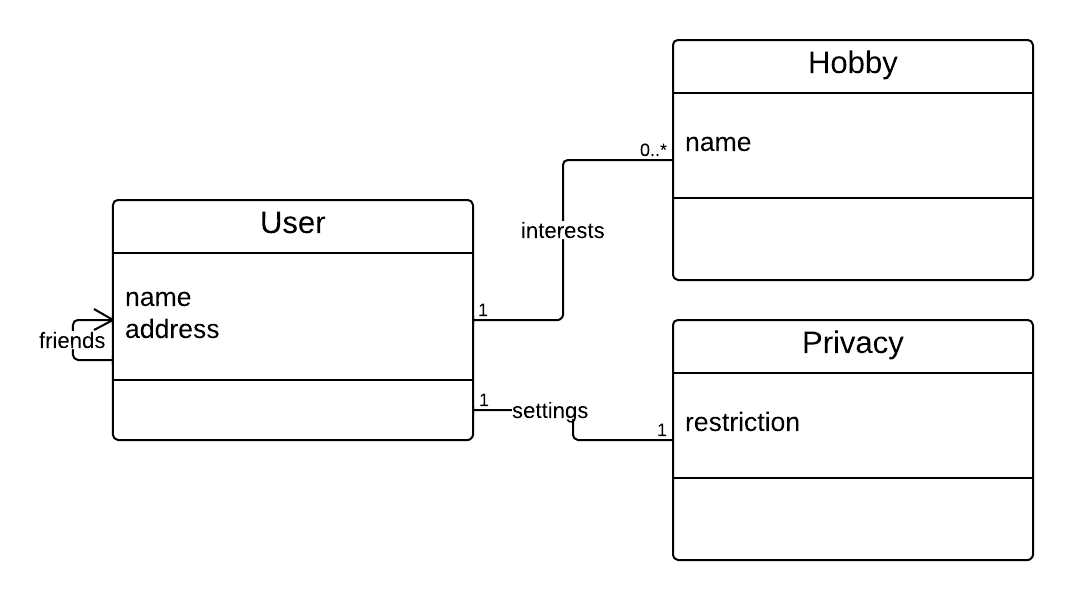
\includegraphics[scale=0.3]{Domain}
\caption{Domain diagram}
\label{fig:domain_diagram}
\end{figure}
\begin{figure}[h!]
\centering
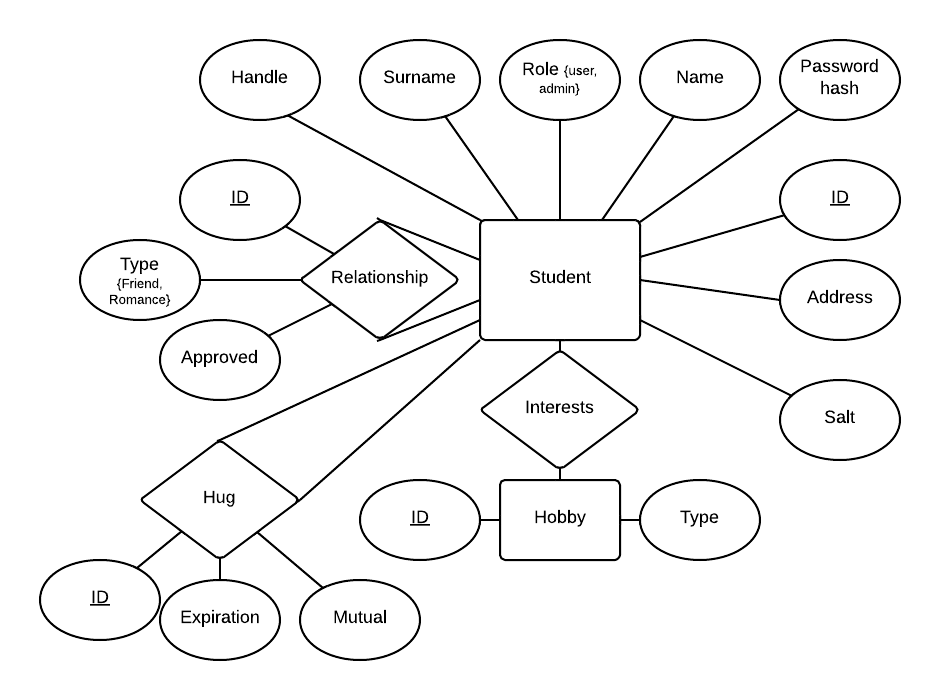
\includegraphics[scale=0.4]{ER}
\caption{Entity relationship diagram of our data-model}
\label{fig:er_diagram}
\end{figure}

\newpage
\subsection{Log file}
\subsubsection{Application online November 1st \label{sec:appendix:online}}
\begin{verbatim}
Nov 1, 2013 9:40:45 AM dk.itu.ssase.hb.beans.LoginBean validateUser
INFO: Authenticated user admin
Nov 1, 2013 9:40:51 AM dk.itu.ssase.hb.listener.AuthPhaseListener afterPhase
INFO: Authorized user
Nov 1, 2013 9:40:51 AM dk.itu.ssase.hb.beans.StudentBean addHobby
INFO: Hobby id: 2
\end{verbatim}

\subsubsection{Race conditions \label{sec:appendix:racecondition}}
\begin{verbatim}
Nov 15, 2013 10:45:55 AM 
dk.itu.ssase.hb.controller.FriendController requestRelationship
INFO: Add relationship to student id: 624
Nov 15, 2013 10:45:55 AM 
dk.itu.ssase.hb.controller.FriendController requestRelationship
INFO: Created relationship request with id: 8

Nov 15, 2013 10:45:56 AM 
dk.itu.ssase.hb.controller.FriendController requestRelationship
INFO: Add relationship to student id: 622
Nov 15, 2013 10:45:56 AM 
dk.itu.ssase.hb.controller.FriendController requestRelationship
INFO: Created relationship request with id: 9

Nov 15, 2013 10:46:01 AM 
dk.itu.ssase.hb.controller.FriendController findUnapprovedRelationshipRequests
INFO: Found friend request from: rasmusgreve
Nov 15, 2013 10:46:01 AM 
dk.itu.ssase.hb.controller.FriendController findUnapprovedRelationshipRequests
INFO: Found friend request from: rasmusgreve

Nov 15, 2013 10:46:32 AM 
dk.itu.ssase.hb.controller.FriendController findUnapprovedRelationshipRequests
INFO: Found friend request from: rasmusgreve
Nov 15, 2013 10:46:32 AM 
dk.itu.ssase.hb.controller.FriendController findUnapprovedRelationshipRequests
INFO: Found friend request from: rasmusgreve

Nov 15, 2013 10:47:40 AM 
dk.itu.ssase.hb.controller.FriendController approveFriend
INFO: Approve relationship id: 9
\end{verbatim}

\subsubsection{Create user}
\begin{verbatim}
dec 15, 2013 3:51:09 AM dk.itu.ssase.hb.beans.CreateStudentBean createUser
INFO: User created with user name newuser
dec 15, 2013 3:51:41 AM dk.itu.ssase.hb.beans.LoginBean validateUser
INFO: Authenticated user newuser
dec 15, 2013 3:51:41 AM dk.itu.ssase.hb.beans.StudentBean findStudentsHobbies
INFO: Found hobbies of the student: 0
dec 15, 2013 3:51:41 AM dk.itu.ssase.hb.beans.StudentBean findAvailableHobbies
INFO: Search for possible hobbies and found 9 results
\end{verbatim}

\subsubsection{Add hobby}
\begin{verbatim}
dec 15, 2013 3:53:22 AM dk.itu.ssase.hb.beans.StudentBean addHobby
INFO: User 4 added Hobby id: 4 
dec 15, 2013 3:53:22 AM dk.itu.ssase.hb.beans.StudentBean findStudentsHobbies
INFO: Found hobbies of the student: 1
dec 15, 2013 3:53:22 AM dk.itu.ssase.hb.beans.StudentBean findAvailableHobbies
INFO: Search for possible hobbies and found 8 results
\end{verbatim}

\subsubsection{Request friendship}
\begin{verbatim}
dec 15, 2013 3:54:50 AM dk.itu.ssase.hb.controller.FriendController 
findNewFriends
INFO: Search for possible friends and found 2 results
dec 15, 2013 3:55:06 AM dk.itu.ssase.hb.controller.FriendController 
requestRelationship
INFO: Add relationship to student id: 3
dec 15, 2013 3:55:06 AM dk.itu.ssase.hb.controller.FriendController 
requestRelationship
INFO: Created relationship request with id: 2
dec 15, 2013 3:55:06 AM dk.itu.ssase.hb.controller.FriendController 
findNewFriends
INFO: Search for possible friends and found 1 results
\end{verbatim}

\subsection{Test reports}
\begin{table}[h!]
\begin{tabular}{| l | l | l | l | l | l | l |}
\hline
Class & Tests & Errors & Failures & Skipped & Success Rate & Time \\ \hline
LoginTest & 2 & 0 & 0 & 0 & 100 \% & 9,411 \\ \hline
\end{tabular}
\end{table}
\begin{table}[h!]
\begin{tabular}{| l | l |}
\hline
testLoginSQLInjection & 8,332 \\ \hline
testLoginXSS & 1,069 \\ \hline
\end{tabular}
\end{table}

\subsection{Hacking}
\begin{figure}[h!]
\centering
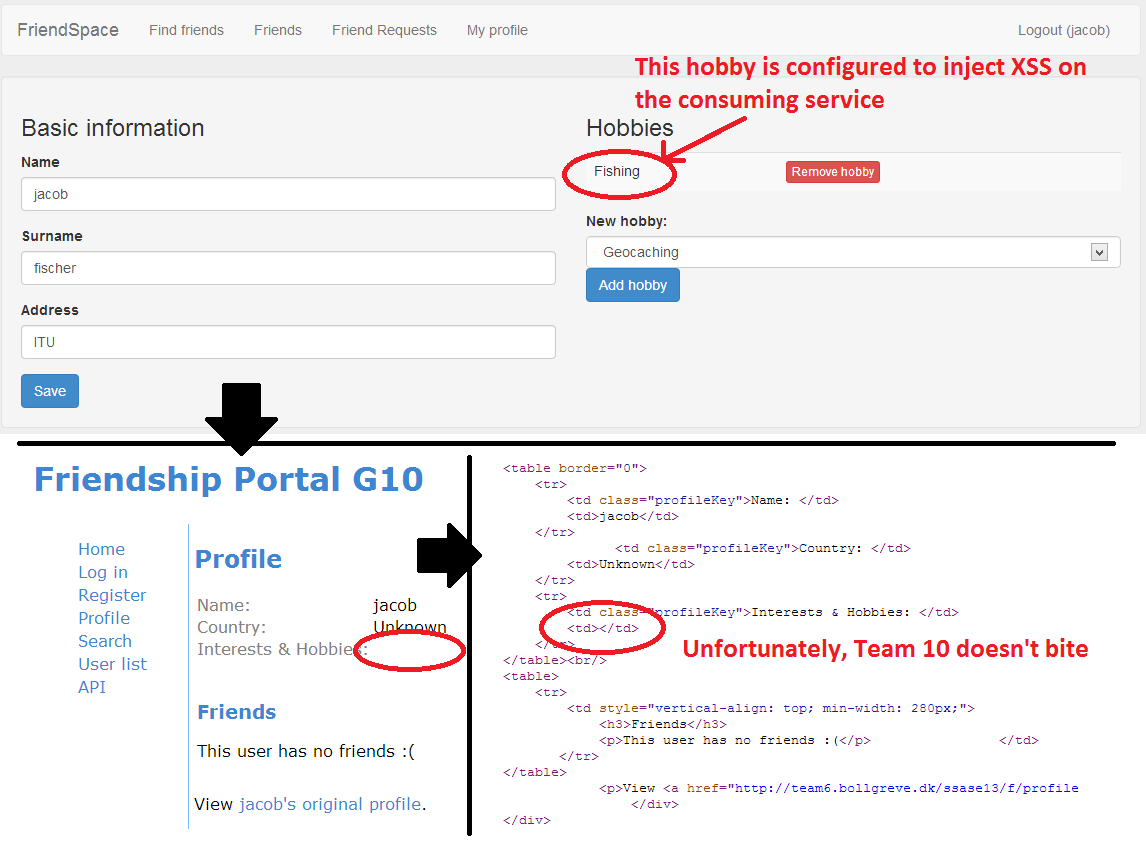
\includegraphics[scale=0.3]{Team10_XSS}
\caption{XSS attack on team 10}
\label{fig:xss_screencap}
\end{figure}

\textbf{Team contract}

The team consists of the following four members:
\begin{itemize}
\item{Jacob Fisher (jaco@itu.dk)}
\item{Christian Lyngbye (clyn@itu.dk)}
\item{Ivaylo Sharkov (isha@itu.dk)}
\item{Rasmus Greve (ragr@itu.dk)}
\end{itemize}
Our expectations of the project is to create a working product with a report meeting all requirements at the right deadlines. We expect to get at least a passing grade and strive towards getting a 10 or 12 at the exam.

We agree on doing project work at least once a week, usually on fridays from 10am to around 2-4pm depending on the amount of work to be done and the deadlines.

Three group members have an exam in week 42. After this, we should be able to meet some Thursdays as well.

Rasmus is having a baby in the end of October and will not be able to do group work on site at ITU in a couple of weeks after this time. He will do work from home and keep in touch with the group via email and instant messaging.

\textbf{Week 37 (13/09/2013)}

Today we created our course log and a git repository.
Jacob retrieved information for our server slice.

We decided on which technologies we were going to use:
We would use the programming language Java and create a Web Application that would use JSF and ORM to map objects to a relational database.

We chose to user a Tomcat server as the application server.

For source control management we have shared a private repository on Github.

We made some agreements in the group regarding collaborative tools.
We chose to use LaTeX to write the report and hosted it on writeLaTeX.
Google Drive for file sharing.
Facebook for communicating outside of the university.

On the server slice we set up a firewall to filter all ports except 6666 which we use for SSH.
We disallowed root access to SSH.
In order to run the application on the server we downloaded and installed: Java JDK, Apache Tomcat and Git.
We discussed how to deploy to the server and considered building the application locally on the server.

We made an initial draft of user stories and requirements for our system.


\textbf{Week 38 (20/09/2013)}

As an experiment Christian installed PostgreSQL on the server slice and it was proved to work so we chose to use it. 
Christian scanned all team servers with nmap and found some differences in solutions e.g. turning ping responses off and closed ports.
Added an example Netbeans project with JSF and started working on connecting to the database.
Rasmus designed the database diagram created an initial creation script for the database.

Ivaylo analyzed the risks.

Planned to do code review and architectural risk analysis.


\textbf{Week 39 (27/09/2013)}

This week we began work on the project report by determining which chapters we need. Jacob started writing the choices of technology chapter and the introductory chapters.

The goal and risk analysis was elaborated on and importet into the report LaTeX document.

We discussed and planned a social engineering attack targeted at all the other groups involving impersonating the TA in an email. We agreed that it was still too early in the process to perform this attack since most teams would be unlikely to have a working webservice to which we could gain access.

\textbf{Week 40 (04/10/2013)}

Ivaylo was sick today and was unable to do group work.

Christian made some refactoring in the codebase requiring the rest of the team to reimport the project into NetBeans.
This refactoring included renaming the project and introducing the Selenide testing framework and a few sample test cases to be elaborated on later. The system is now called ``FriendSpace''.

Rasmus spent a bit of time styling the webpages using Twitter Bootstrap. Jacob drew a logo to make the visual expression of the webpages more appealing.

The system was deployed to the webserver on port 80 which was opened. Accessing the root of the server redirects the user to /ssase13.

Furthermore, the team spent a lot of time throughout the day finishing up the first draft of the report for the first hand-in.


\textbf{Week 41 (11/10/2013)}


\textbf{Week 42 (18/10/2013)}


\textbf{Week 43 (25/10/2013)}

Worked on Sins presentation about Race Conditions. This led to some improvements of our code.

\textbf{Week 44 (01/11/2013)}
\textbf{Week 45 (08/11/2013)}

Reorganized the report into distinct sections.
Divided work between us to help organize.

\textbf{Week 46 (15/11/2013)}

Implemented friend requests.
Rewrote risk analysis to use the book structure.

\end{document}
